\subsubsection{Statistical Physics: Dynamical Processes on Complex
Networks} \index{Meyer-Ortmanns, Hildegard}

\paragraph{Research Team} Hildegard Meyer-Ortmanns (Professor), Xiang Li (Humboldt Fellow),
Filippo Radicchi (Research Associate), Daniele Vilone
(Postdoctoral Fellow), Sooyeon Yoon (Visiting Graduate Student), Yeong-Yeol Ahn (Visiting Graduate Student)\\
\\
Recently, applications of statistical physics to networks became
quite topical. The networks range from genetic, proteomic,
metabolic and neural systems to social systems as well as
artificial ones like the worldwide web and the internet. Apart
from static properties there are also dynamical processes in
common to these networks such as spreading or cooperation
phenomena, or self-organization of individual units. For example,
spreading viruses may refer to diseases in social systems as well
as to computer viruses spreading in the internet. An example for
cooperation and self-organization is the formation of synchronized
clusters in an ensemble of oscillators, similar to an ensemble of
clocks.
\\
We are studying evolutionary aspects of such networks, their
approach to stationary states, pattern formation and the
dependence on the network topology.


\paragraph{Highlights}
{\it Evolutionary Algorithms}
The reduction of frustration is the driving force in a number of
natural and artificial processes. "Frustration" is a concept that
is familiar from the psychological or social context. In a social
system a state that is characterized by frustration is called
imbalanced. Such a situation arises, for example, when one
individual has two friends who are mutually enemies. In physics
the notion of frustration is familiar from spin systems. If there
is competition between ferromagnetic and antiferromagnetic
interactions, it may happen that some bonds remain unsatisfied
whatever value certain spins take. Also in optimization problems
of computer science "frustration" may arise when not all logical
constraints between say Boolean variables can be satisfied
simultaneously. Interestingly, although the examples are taken
from very different areas, the mathematical criterion to test on
the degree of frustration is the same. In \cite{ortmanns1} we
studied the approach to social balance on a diluted network whose
nodes are individuals and whose edges are relationships between
these individuals. We determined the phase structure of this
system, the stationary states (in physical terms absorbing and
non-absorbing states) and the size dependence of the time to reach
these states. In particular we could answer the question as to
whether appropriate local (individual) behavior can ensure that
the stationary state with zero degree of frustration is reached
within a finite lifetime. The answer is that it depends on the
individual tendency to turn a relationship into friendship (in
mathematical terms: to flip the sign of the spin from $-$ to $+$).
Moreover we have shown that the approach to social balance can be
uniquely mapped to the solution of a so-called satisfiability
problem in computer science. Here a similar question is posed: can
a local stochastic algorithm find a solution, which is known to
exist, within a finite time? (If not, the algorithm would be
useless.)
Again the answer depends on the parameter choice for this local algorithm. \\
These examples nicely illustrate the existence of common problems
and common solutions in very different networks whenever the
mathematical structure is the same (as it was here the criterion
for identifying and reducing frustration). \\The results mentioned
so far were obtained on a random, diluted network topology. On a
regular, triangular topology the reduction of frustration
always ends up in an absorbing (frozen) state, but the time to
reach this state grows linearly or power-like, depending on the
phase. The phase transition itself can be described in terms of a
percolation picture with critical exponents of a new universality
class, as we have shown in \cite{ortmanns2}. Our main motivation
behind these studies is the identification of the same driving
evolutionary mechanism in natural systems like genetic ones. For
genetic systems it has been speculated that it is the low degree
of frustration that is responsible for the low number of stable
cell states. \vskip5pt {\it Synchronization} In continuation of our former work on
synchronization of oscillators \cite{ortmanns3} we studied
dynamically induced pacemakers. In biological systems two kind of
pacemakers are found: pacemakers which are different and
distinguished from the set of oscillators which they entrain, and
pacemakers of the same oscillatory type, but getting dynamically
established in their role of entraining the others. In
\cite{ortmanns4} we found out that the oscillators with the
largest natural frequency in a system with a linear gradient of
natural frequencies becomes the pacemaker in a dynamically induced
way. "Pacemaker" is understood in the sense that the oscillator
becomes the center of circular waves on the lattice of
oscillators. Here the waves refer to the oscillator's phases, see
figure \ref{fig:ortmanns}. Due to the reflection and interference
of waves in intermediate states, patterns in phase space form, as
they are experimentally known from concentration patterns in
certain chemical reactions.


\begin{figure}[ht]
  \begin{center}
    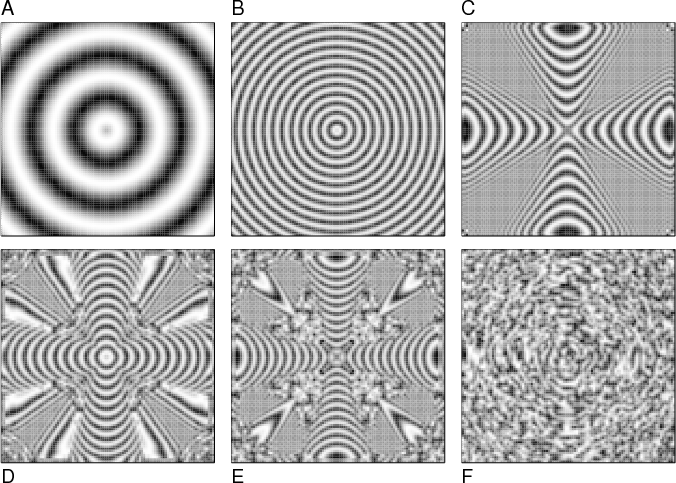
\includegraphics[width=\hsize]{Ortmanns/ortmanns2.png}
    \mycaption{Stationary patterns in the phases of oscillators that are posed on a square lattice.
The various snapshots correspond to different degrees of partial synchronization.)}\label{fig:ortmanns}
   \end{center}
\end{figure}

\paragraph{Organization}
% list the (research) events you have organized, if any,

\begin{enumerate}
\item  International Center for Transdisciplinary Studies (ICTS),
scientific coordination (with B.\ Kramer and P.\ Schupp) and
organization of seminars 2006
\end{enumerate}

\paragraph{Collaborations}
\begin{enumerate}
\item {\sl Kyung Hee University, Seoul (Korea)}\\ Prof. Soon-Hyung
Yook\\ Percolation theory and epidemic spreading
\item  {\sl Technische Universit\"at Hamburg Harburg}\\ Prof. An-Ping Zeng\\
Autocatalytic Sets and Metabolic Networks \item{\sl Korea
Institute of Advanced Science and Technology, Daejeon,
Korea}\\Yong Yeol Ahn\\ Neural Network Models for the Visual
Cortex of the Monkey
\item{\sl Humboldt University Berlin}\\Prof.Michael Zaks\\
Dynamics of Excitable Media \item {\sl Bremen University} \\Prof.
Stefan Bornholdt\\Boolean Networks
\item {\sl Jacobs University Bremen}\\
Prof. Marc-Thorsten H\"utt\\Genetic
Networks; \\Prof. Claus Hilgetag\\Neural Networks
\end{enumerate}


\paragraph{Grants}
% list the running grants in 2005, if none have been received, please delete this
% subsection.
\begin{enumerate}
\item PhD-position, DFG-Grant ME 1332/10-2
\item Fellowship, Humboldt-Stiftung IV-CHN/1116658 STP
\item 2 DAAD grants (Germany-Korea): a)``Physics of Surface Growth'', b) ``Neural
  Networks''  
\end{enumerate}


\paragraph{Awards, Prizes}
% list the grants you have received in 2005, if none have been received, please delete this
% subsection.
\begin{enumerate}
\item W.E.Heraeus-summer school on {\it Interfaces between Physics
and Computer Science} to take place in June 2007, approved in 2006
\item W.E.Heraeus-summer school on {\it Statistical Physics of
Gene Regulation: From Genetic Networks to Expression Data and Back
} (organized with M.T.H\"utt) to take place in July 2007, approved in 2006
\end{enumerate}

\nocite{ortmanns0}
\nocite{ortmanns5}
\nocite{ortmanns6}
\nocite{meyerortmanns1}
\nocite{vilone1}
